%-------------------------------------------------------------------------------
% Constrói a capa com base na seção de identificação do main.tex
%-------------------------------------------------------------------------------
\begin{capa}
    \setlength{\belowcaptionskip}{0pt}
    \setlength{\abovecaptionskip}{0pt}
    \setlength{\intextsep}{-18pt}
        \begin{figure}[h]
        \begin{center}
            \includegraphics[scale=1.0]{img/LOGO_UNIVASF_big.pdf}
        \end{center}
      \end{figure}

        %\includegraphics[scale=0.6]{img/univasf.jpg}
        \center
      {\ABNTEXchapterfont\large\imprimirinstituicao}

      \vspace*{2cm}
          {\imprimirautor}
      \vspace*{2cm}
        \begin{center}
        \ABNTEXchapterfont\bfseries\large\imprimirtitulo
        \end{center}
      \vfill

      \ABNTEXchapterfont\bfseries\large\imprimirlocal\\
      \the\year

      \vspace*{1cm}
\end{capa}
%-------------------------------------------------------------------------------
% Constrói a folha de rosto com base na seção de identificação do main.tex
%-------------------------------------------------------------------------------
\begin{folhaderosto}
    \center
      {\ABNTEXchapterfont\large\imprimirinstituicao}

    \vspace*{2cm}
          {\imprimirautor}
      \vspace*{2cm}
    \vspace*{\fill}

    {\ABNTEXchapterfont\bfseries\large\imprimirtitulo}
    \vspace*{\fill}

    {\hspace{.45\textwidth}
    \begin{minipage}{.5\textwidth}
      \SingleSpacing
      \imprimirpreambulo \\ \\

      {\imprimirorientadorRotulo~\imprimirorientador\par}
      {\imprimircoorientadorRotulo~\imprimircoorientador\par}

    \end{minipage}%
    \vspace*{\fill}}%
    \vspace*{\fill}
      \ABNTEXchapterfont\bfseries\large\imprimirlocal\\
      \the\year
    \vspace*{1cm}
\end{folhaderosto}

%-------------------------------------------------------------------------------
% Constrói a ficha catalográfia com base na seção de identificação do main.tex
% Está comentado porque no final das contas a biblioteca do seu campus que gera a
% numeração, você pode adicionar os numeros aqui, ou anexar o pdf gerado por eles
% ao documento.
%-------------------------------------------------------------------------------
%\begin{fichacatalografica}
%	\vspace*{\fill}					% Posição vertical
%	\hrule							% Linha horizontal
%	\begin{center}					% Minipage Centralizado
%	\begin{minipage}[c]{12.5cm}		% Largura
%
%	\imprimirautor
%
%	\hspace{0.5cm} \imprimirtitulo  / \imprimirautor. --
%	\imprimirlocal, \the\year-
%
%	\hspace{0.5cm} xx p. : il. (algumas color.) ; 30 cm.\\
%
%	\hspace{0.5cm} \imprimirorientadorRotulo~\imprimirorientador\\
%
%	\hspace{0.5cm}
%	\parbox[t]{\textwidth}{\imprimirtipotrabalho~--~\imprimirinstituicao,
%	\the\year.}\\
%
%	\hspace{0.5cm}
%		1. Palavra-chave1.
%		2. Palavra-chave2.
%		I. Orientador.
%		II. Universidade xxx.
%		III. Faculdade de xxx.
%		IV. Título\\
%
%	\hspace{8.75cm} CDU 02:141:005.7\\
%
%	\end{minipage}
%	\end{center}
%	\hrule
%\end{fichacatalografica}

%--------------------------------------------------------------------------------
% Anexando a ficha catalogáfica e a folha de aprovação
%--------------------------------------------------------------------------------
% 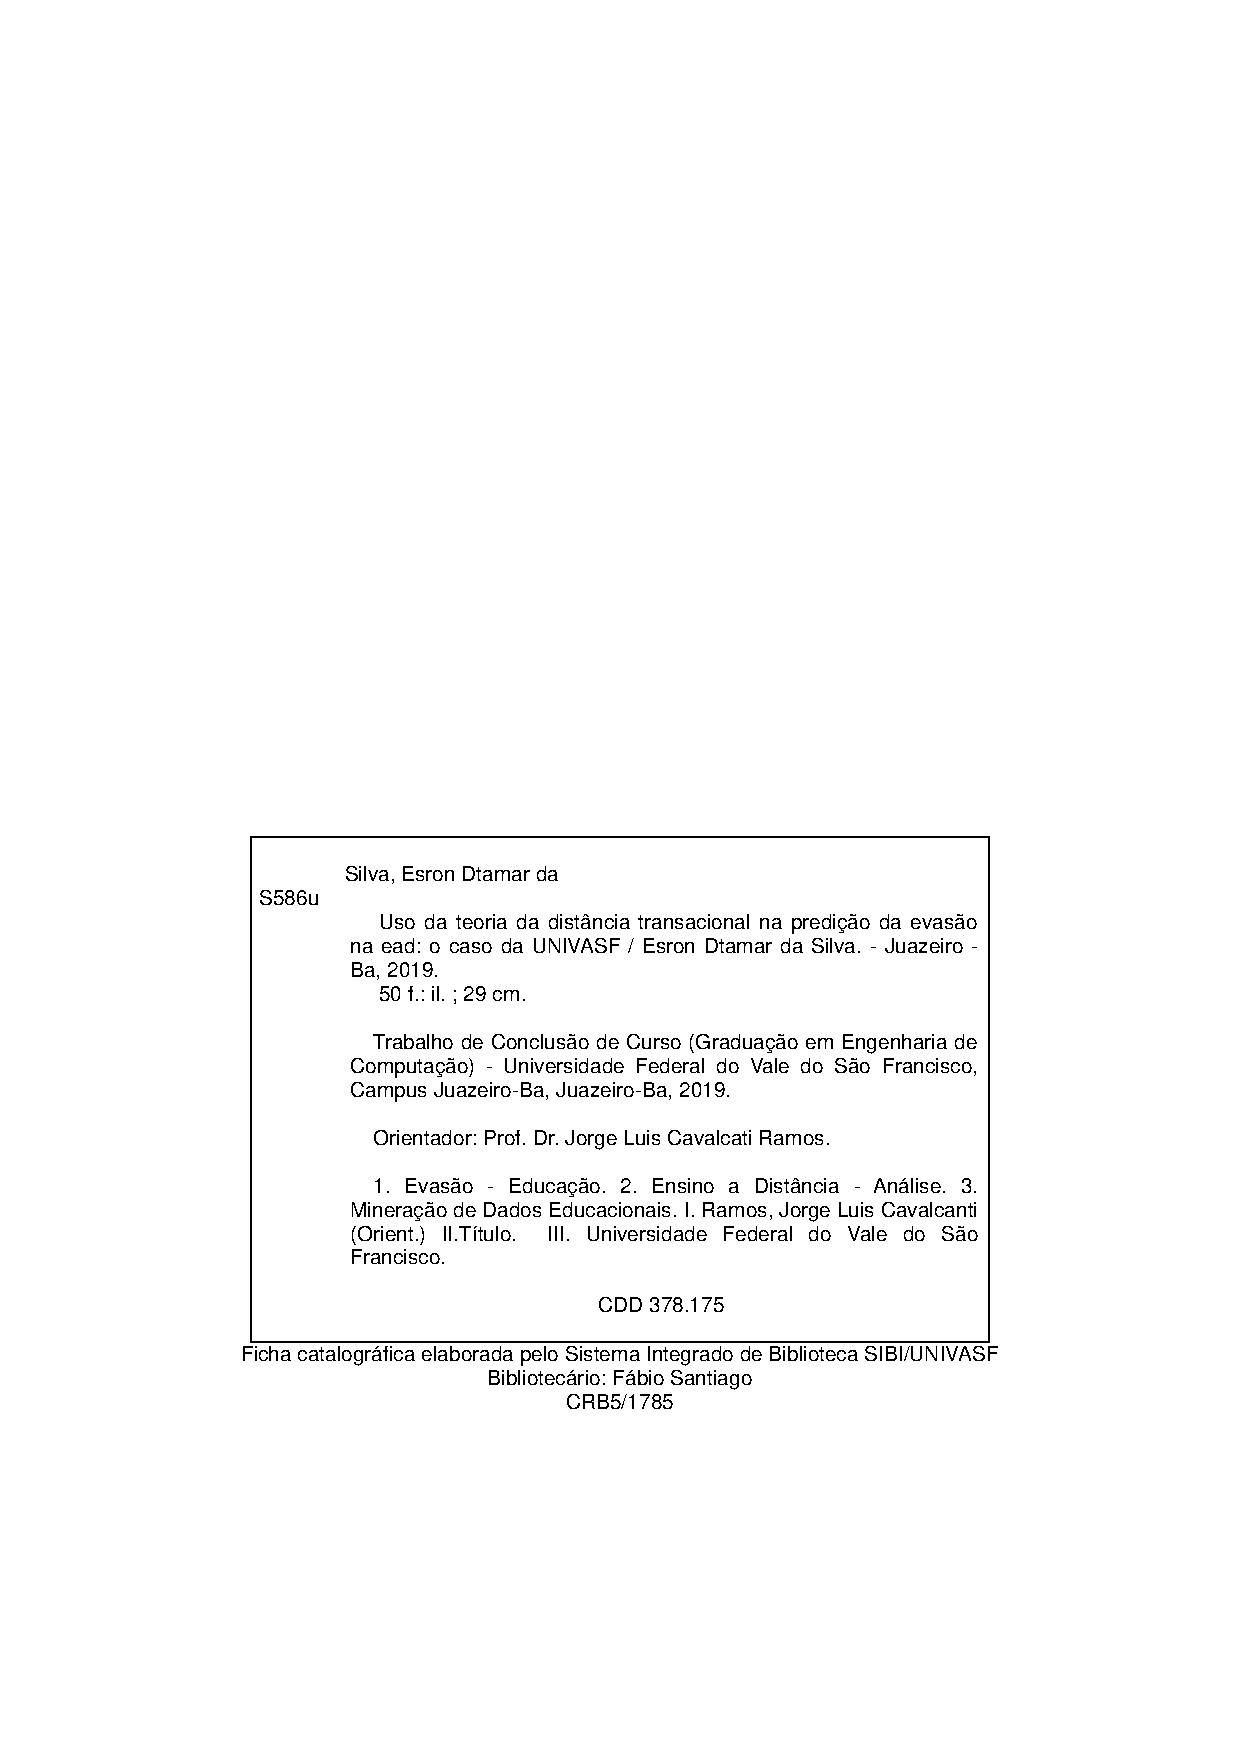
\includepdf[pages=-]{anexos/ficha.pdf}

% 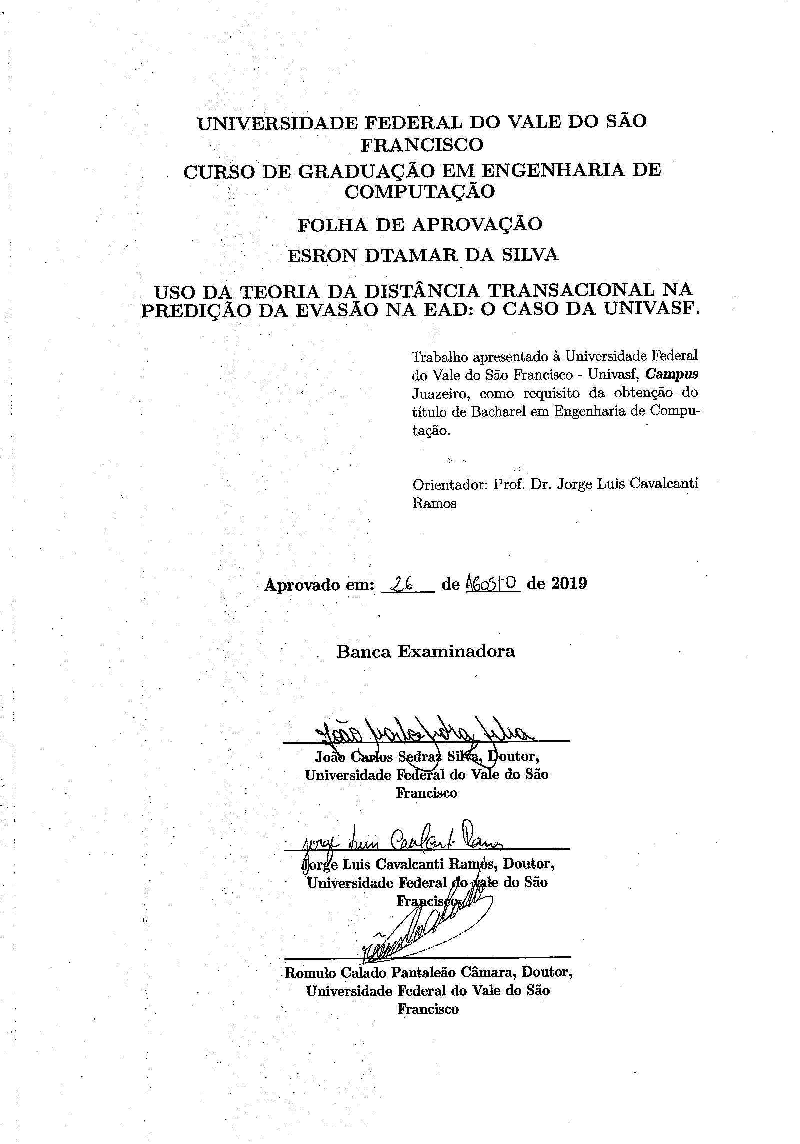
\includepdf[pages=-]{anexos/aprovacao.pdf}

% \setlength{\ABNTEXsignwidth}{12cm}

%--------------------------------------------------------------------------------
% Está comentado pelo mesmo motivo da ficha catalográfica
%--------------------------------------------------------------------------------
%\begin{folhadeaprovacao}
%	\begin{center}
%	    {\ABNTEXchapterfont\bfseries\large\imprimirinstituicao}
%	    \vspace*{\fill}
%
%	    {\ABNTEXchapterfont\bfseries\large FOLHA DE APROVAÇÃO}
%	    \vspace*{\fill}
%
%	    {\ABNTEXchapterfont\bfseries\large\imprimirautor}
%
%	    \vspace*{\fill}\vspace*{\fill}
%	    {\ABNTEXchapterfont\bfseries\large\imprimirtitulo}
%	    \vspace*{\fill}
%
%	    {\hspace{.45\textwidth}
%		\begin{minipage}{.5\textwidth}
%			\SingleSpacing
%			\ABNTEXchapterfont\imprimirpreambulo \\ \\
%
%			{\ABNTEXchapterfont\imprimirorientadorRotulo~\imprimirorientador\par}
%			{\ABNTEXchapterfont\imprimircoorientadorRotulo~\imprimircoorientador\par}
%
%		\end{minipage}%
%	    \vspace*{\fill}}
%	\end{center}
%
%	\vspace*{\fill}
%
%	\begin{center}
%			 \ABNTEXchapterfont\large Aprovado em: \_\_\_\_ de \_\_\_\_ de 2017
%	\end{center}

%	\vspace*{\fill}

%	\begin{center}
%			 \ABNTEXchapterfont\bfseries\large Banca Examinadora
%	\end{center}
%
%   \ABNTEXchapterfont\assinatura{Fábio Nelson de Sousa Pereira, Mestre, Universidade Federal do Vale do São Francisco}
%	\ABNTEXchapterfont\assinatura{Jorge Luis Cavalcanti Ramos, Doutor, Universidade Federal do vale do São Francisco}
%  \ABNTEXchapterfont\assinatura{Ricardo Argenton Ramos, Doutor, Universidade Federal do Vale do São Francisco}
%	 \vspace*{\fill}


%\end{folhadeaprovacao}

%-------------------------------------------------------------------------------
% Insere a epígrafe
%-------------------------------------------------------------------------------
% \newpage
% \vspace*{\fill}
% \begin{flushright}
%     \textit{Lorem Ipsum...}
% \end{flushright}

%-------------------------------------------------------------------------------
% Seção de agradecimentos
%-------------------------------------------------------------------------------
% \begin{agradecimentos}

% \lipsum[2-4]

% \end{agradecimentos}

%-------------------------------------------------------------------------------
% Insere a segunda epígrafe
%-------------------------------------------------------------------------------
% \begin{epigrafe}
%   \vspace*{\fill}
%   \begin{flushright}
%     Se pude enxergar a tão grande distância, foi subindo nos ombros de gigantes.\\
%      \vspace{\baselineskip}
%     \textbf{Isaac Newton}\\
%     \textbf{Carta à Robert Hooke, 1676}
%   \end{flushright}
% \end{epigrafe}



%-------------------------------------------------------------------------------
% Seção de resumos
%-------------------------------------------------------------------------------
% resumo em português
\setlength{\absparsep}{18pt} % ajusta o espaçamento dos parágrafos do resumo
\begin{resumo}

  Os avanços do acesso às tecnologias da informação criou um ambiente fértil
  para a pesquisa na área de educação a distância (EAD). Porém, apesar da grande
  disponibilidade e flexibilidade, os cursos da modalidade EAD, no Brasil, ainda
  sofrem com o problema da evasão de estudantes. Acompanhando o crescimento da
  EAD, se desenvolve também a área de Mineração de Dados Educacionais (MDE).
  Este trabalho propõe a utilização de uma metodologia fundamentada em técnicas
  de MDE com o objetivo de construir e avaliar modelos de classificação da
  situação final de estudantes da EAD entre duas classes, evadidos e não
  evadidos usando os algoritmos de aprendizagem de máquina: KNN, Regressão
  Logística e Árvore de Decisisão. Na construção dos modelos, foram utilizados
  dados obtidos de duas turmas no contexto da Universidade Federal do Vale do
  São Francisco (UNIVASF), e, alem disso, as variáveis preditoras foram
  concebidas a partir dos construtos da Teoria da Distância Transacional (TDT).
  Os resultados apontam que essas variáveis podem ser usadas como fontes de
  dados dos classificadores, alcançando valores similares ao estudo original que
  deu origem à este trabalho e em relação aos verificados em trabalhos
  similares.

  \textbf{Palavras-chave}: Ciencia de Dados. Aprendizagem Supervisionada. Evasao. Descoberta de Conhecimentos em Bases de Dados

\end{resumo}
\newpage

% resumo em inglês
\begin{resumo}[Abstract]
\begin{otherlanguage*}{english}

  The advances in information technologies created a very fertile research
  environment in the distance education field. However, despite of the great
  disponibility and flexibility, the brazilian DE course genre still suffers
  from the problem of student dropout. Along with the growing in DE, the
  Educational Data Mining (EDM) is developing as well. This paper proposes the
  use of a methodology based on EDM techniques with the purpose of constructing
  and evaluating classification models of situation of distance learning
  students between two classes, evaded and not evaded using machine learning
  algorithms: KNN, Logistic Regression and Decision Tree. In the construction of
  the models, we used data obtained from two classes in the context of the
  Federal University of Vale do Francisco (UNIVASF), and, moreover, the
  predictor variables were conceived from the Transactional Distance Theory
  (TDT) constructs. The results indicate that these variables can be used as
  sources of data from the classifiersm reaching values similar to the
  original study that gave rise to this work and in relation to those verified
  in similar.

  \textbf{Key-words}: Data Science. Supervised Learning. Knowledge Discovery in Databases

\end{otherlanguage*}
\end{resumo}


%-------------------------------------------------------------------------------
% Insere lista de ilustrações
%-------------------------------------------------------------------------------
\begin{KeepFromToc} % Este comando evita que todas as seções dentro dele de apareçam no sumário
\pdfbookmark[0]{\listfigurename}{lof}
\listoffigures
\cleardoublepage


%-------------------------------------------------------------------------------
% Insere lista de tabelas
%-------------------------------------------------------------------------------
\pdfbookmark[0]{\listtablename}{lot}
\listoftables
\cleardoublepage

%-------------------------------------------------------------------------------
% Insere lista de quadros
%-------------------------------------------------------------------------------
\pdfbookmark[0]{\listofquadrosname}{loq}
\listofquadros*
\cleardoublepage

%-------------------------------------------------------------------------------
% Ajusta lista de código - alterar de figures para códigos - by @Gabrielr2508
%-------------------------------------------------------------------------------
% \makeatletter
% \let\l@listing\l@figure
% \def\newfloat@listoflisting@hook{\let\figurename\listingname}
% \makeatother

%-------------------------------------------------------------------------------
% Insere lista de códigos - by @leolleocomp
%-------------------------------------------------------------------------------
% \listoflistings

\end{KeepFromToc}

%-------------------------------------------------------------------------------
% Insere lista de abreviaturas e siglas
%-------------------------------------------------------------------------------
\begin{siglas}
  \item[ABED] Associação Brasileira de Educação a Distância
  \item[AVA] Ambiente Virtual de Aprendizagem
  \item[CFA] Análise Fatorial Confirmatória
  \item[CSV] \textit{Comma Separeted Value}
  \item[DM] \textit{Data Mining}
  \item[DT] Distância Transacional
  \item[EAD] Educação a Distância
  \item[EDM] \textit{Educational Data Mining}
  \item[IDE] \textit{Integrated Development Environment}
  \item[IES] Instituição de ensino superior
  \item[INEP] Instituto Nacional de Estudos e Pesquisas Educacionais Anísio Teixeira
  \item[KDD] \textit{Knowledge Discovery in Databases}
  \item[KNN] \textit{K-nearest Neighbors}
  \item[LA] \textit{Learning Analytics}
  \item[LMS] \textit{Learning Management System}
  \item[ML] \textit{Machine Learning}
  \item[RL] Regressão Logística
  \item[SEAD] Secretaria de Educaçao a Distância
  \item[SGBD] Sistema de Gerenciamento de Banco de Dados
  \item[SQL] \textit{Structured Query Language}
  \item[STI] Secretaria de Tecnologia da Informação
  \item[SVM] \textit{Support Vector Machine}
  \item[TCC II] Trabalho de Conclusão de Curso II
  \item[TDT] Teoria da Distância Transacional
  \item[UNIVASF] Universidade Federal do Vale do São Francisco
\end{siglas}

%-------------------------------------------------------------------------------
% Insere o sumario
%-------------------------------------------------------------------------------
\pdfbookmark[0]{\contentsname}{toc}
\tableofcontents*
\cleardoublepage
